The learnAir V1 sensor was first installed on April 6th, 2016 and taken down on April 14th.  This preliminary test resulted in serious sensor corrosion and unuseable data.

The useful section of the co-location test ran from April 15th to June 13th (59 days).  During that time, several tests were performed.  In total we validated 8 different sensors representing 6 distinct sensor types over periods ranging from 21 to 59 days.  Our co-located test sets range from 1,431 samples of hourly data up to 85,739 samples of minute-resolved data.  


\begin{figure}[htb]
 	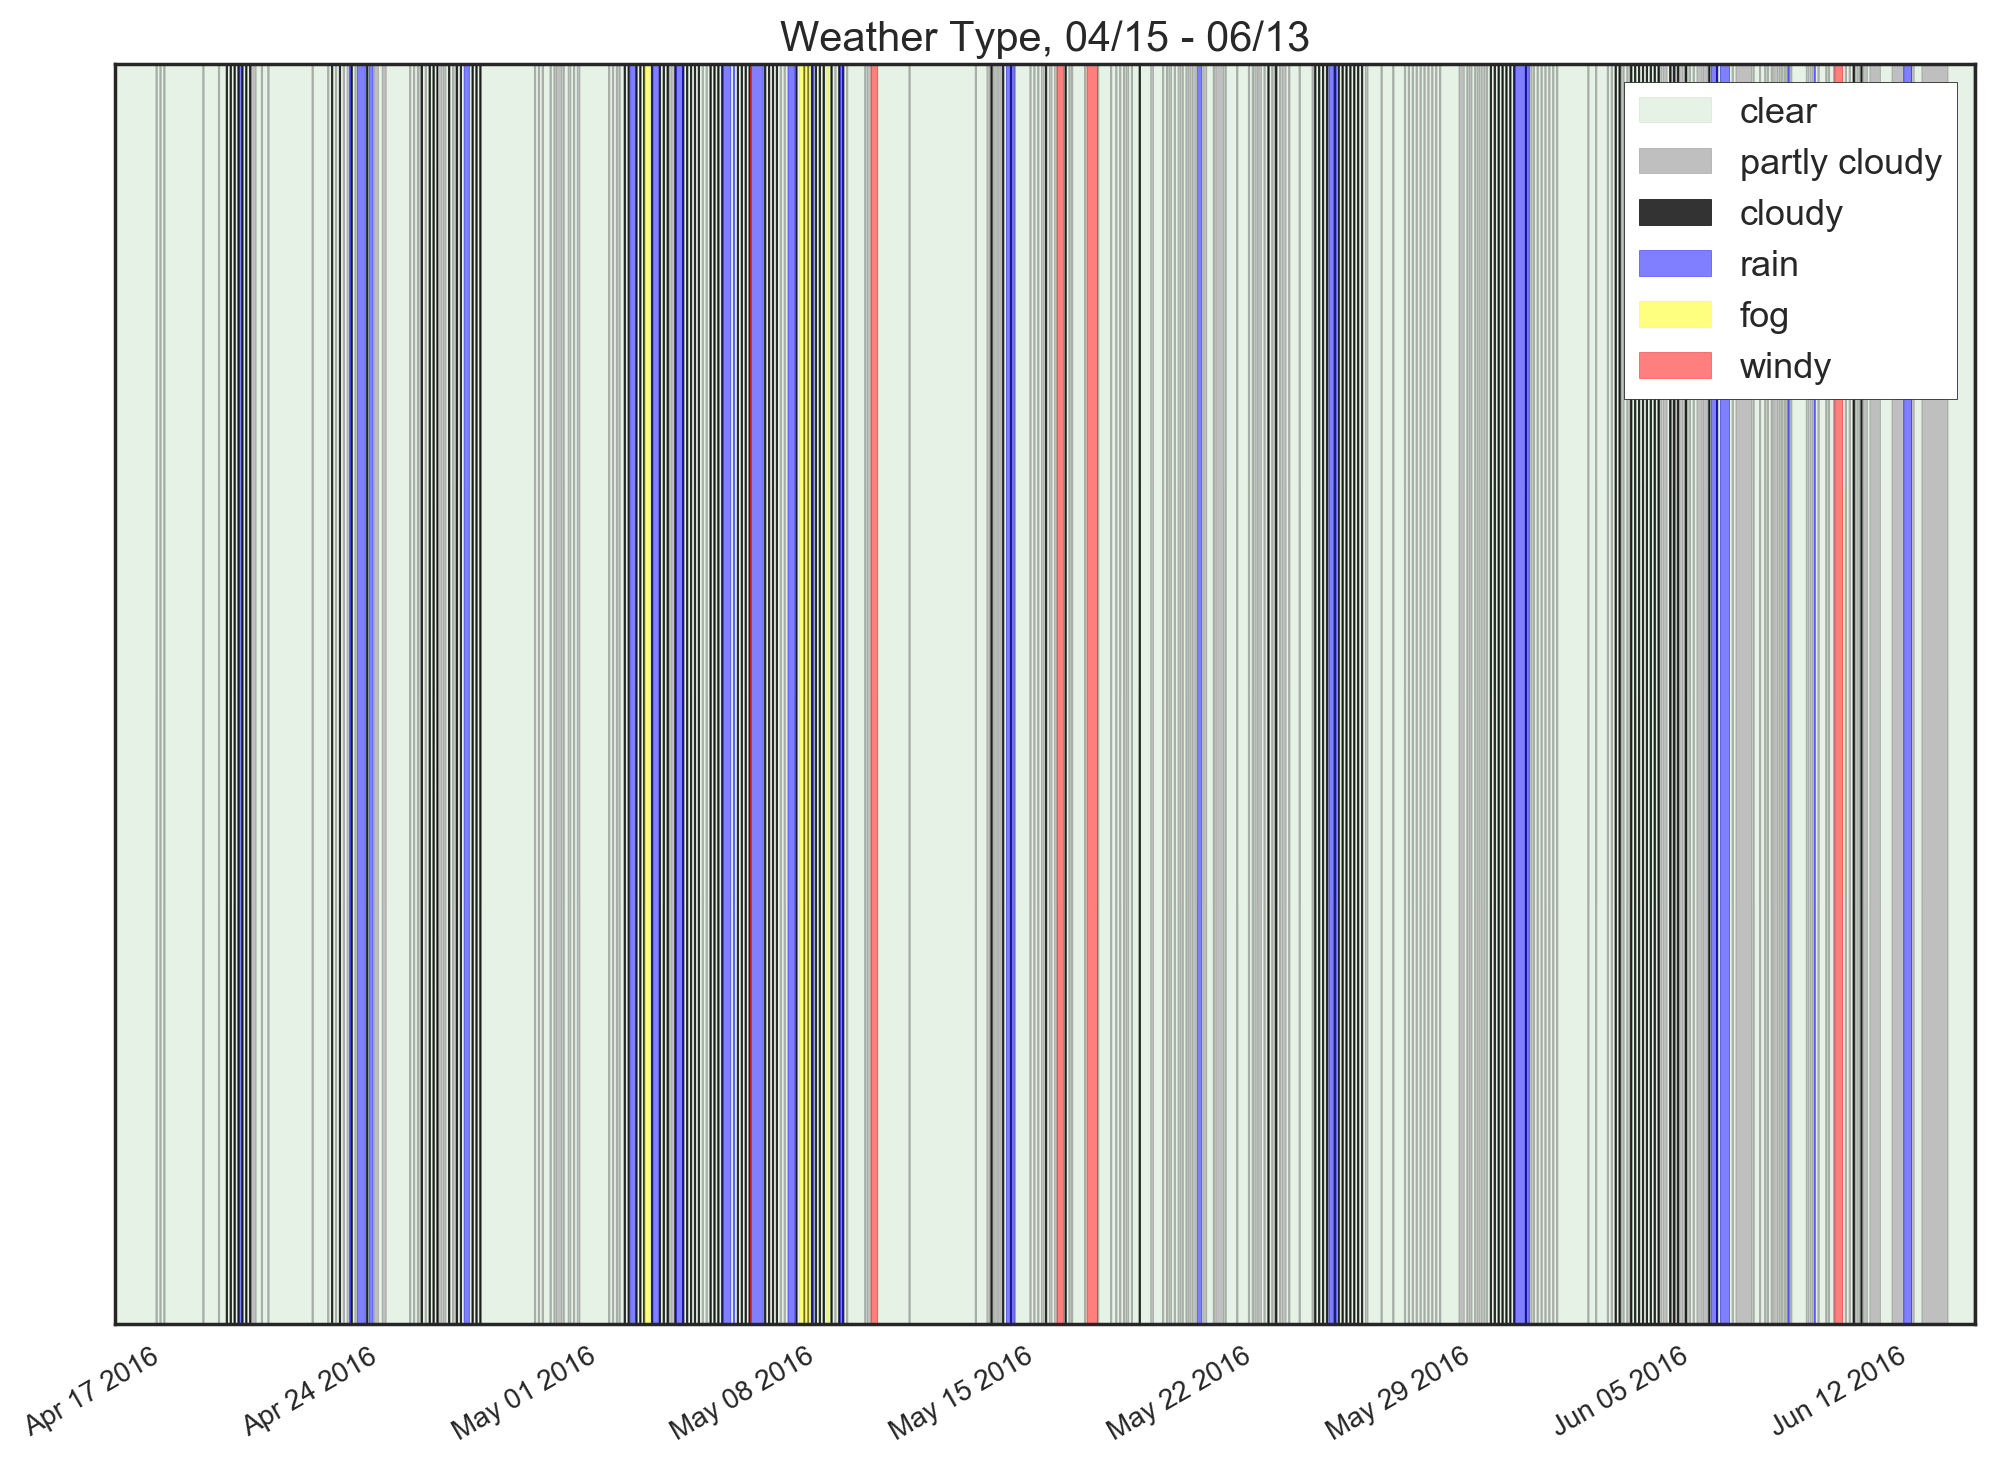
\includegraphics[width=\textwidth-0.5cm]{figs/weather}               
 	 \caption{Weather during Test Period.}
  	\label{fig:weather}
\end{figure}


From April 15th through May 23rd (38 days with one 40 minute service break), an older set of AlphaSense O3 and CO electrochemical gas sensors were characterized.  This set was calibrated in Dec 2013 (2 years, 4 months old calibration at the start of the test).  55,589 samples of minute-resolution data was collected to characterize these sensors.

From May 23rd to June 13th (21 days), a brand new set of AlphaSense O3+NO2, NO2, and CO electrochemical gas sensors were characterized (5 month old calibration at the start of the test).  30,150 samples were collected to characterize these sensors.

The two tests of an older and newer set of the same type of Alphasense sensors (O3 and CO) can provide interesting insights-- by comparing the data between the two tests we may be able to draw insights into age- and use-related differences.  By combining the two sets after calibration, we have a long set of data spanning several months to test predictive techniques with.  Assuming the underlying failure modes are the same for sensors of the same make/model, this combined set should be useful at providing insight into the underlying device mechanics.

From April 15th through June 6th (52 days, with two 40 minute service outages), a new SmartCitizen sensor-- with its NO2 and CO sensors-- was installed and running at the MassDEP site.  This sensor gave 85,739 minute-resolved samples.

Finally, from April 15th through June 13th (59 days), our Sharp Particulate Sensor collected samples that we resolved to 1 hour intervals, to match the MassDEP BAM reference.  1,431 samples were collected from this technique.  

\FloatBarrier
\begin{figure}[htb]
 	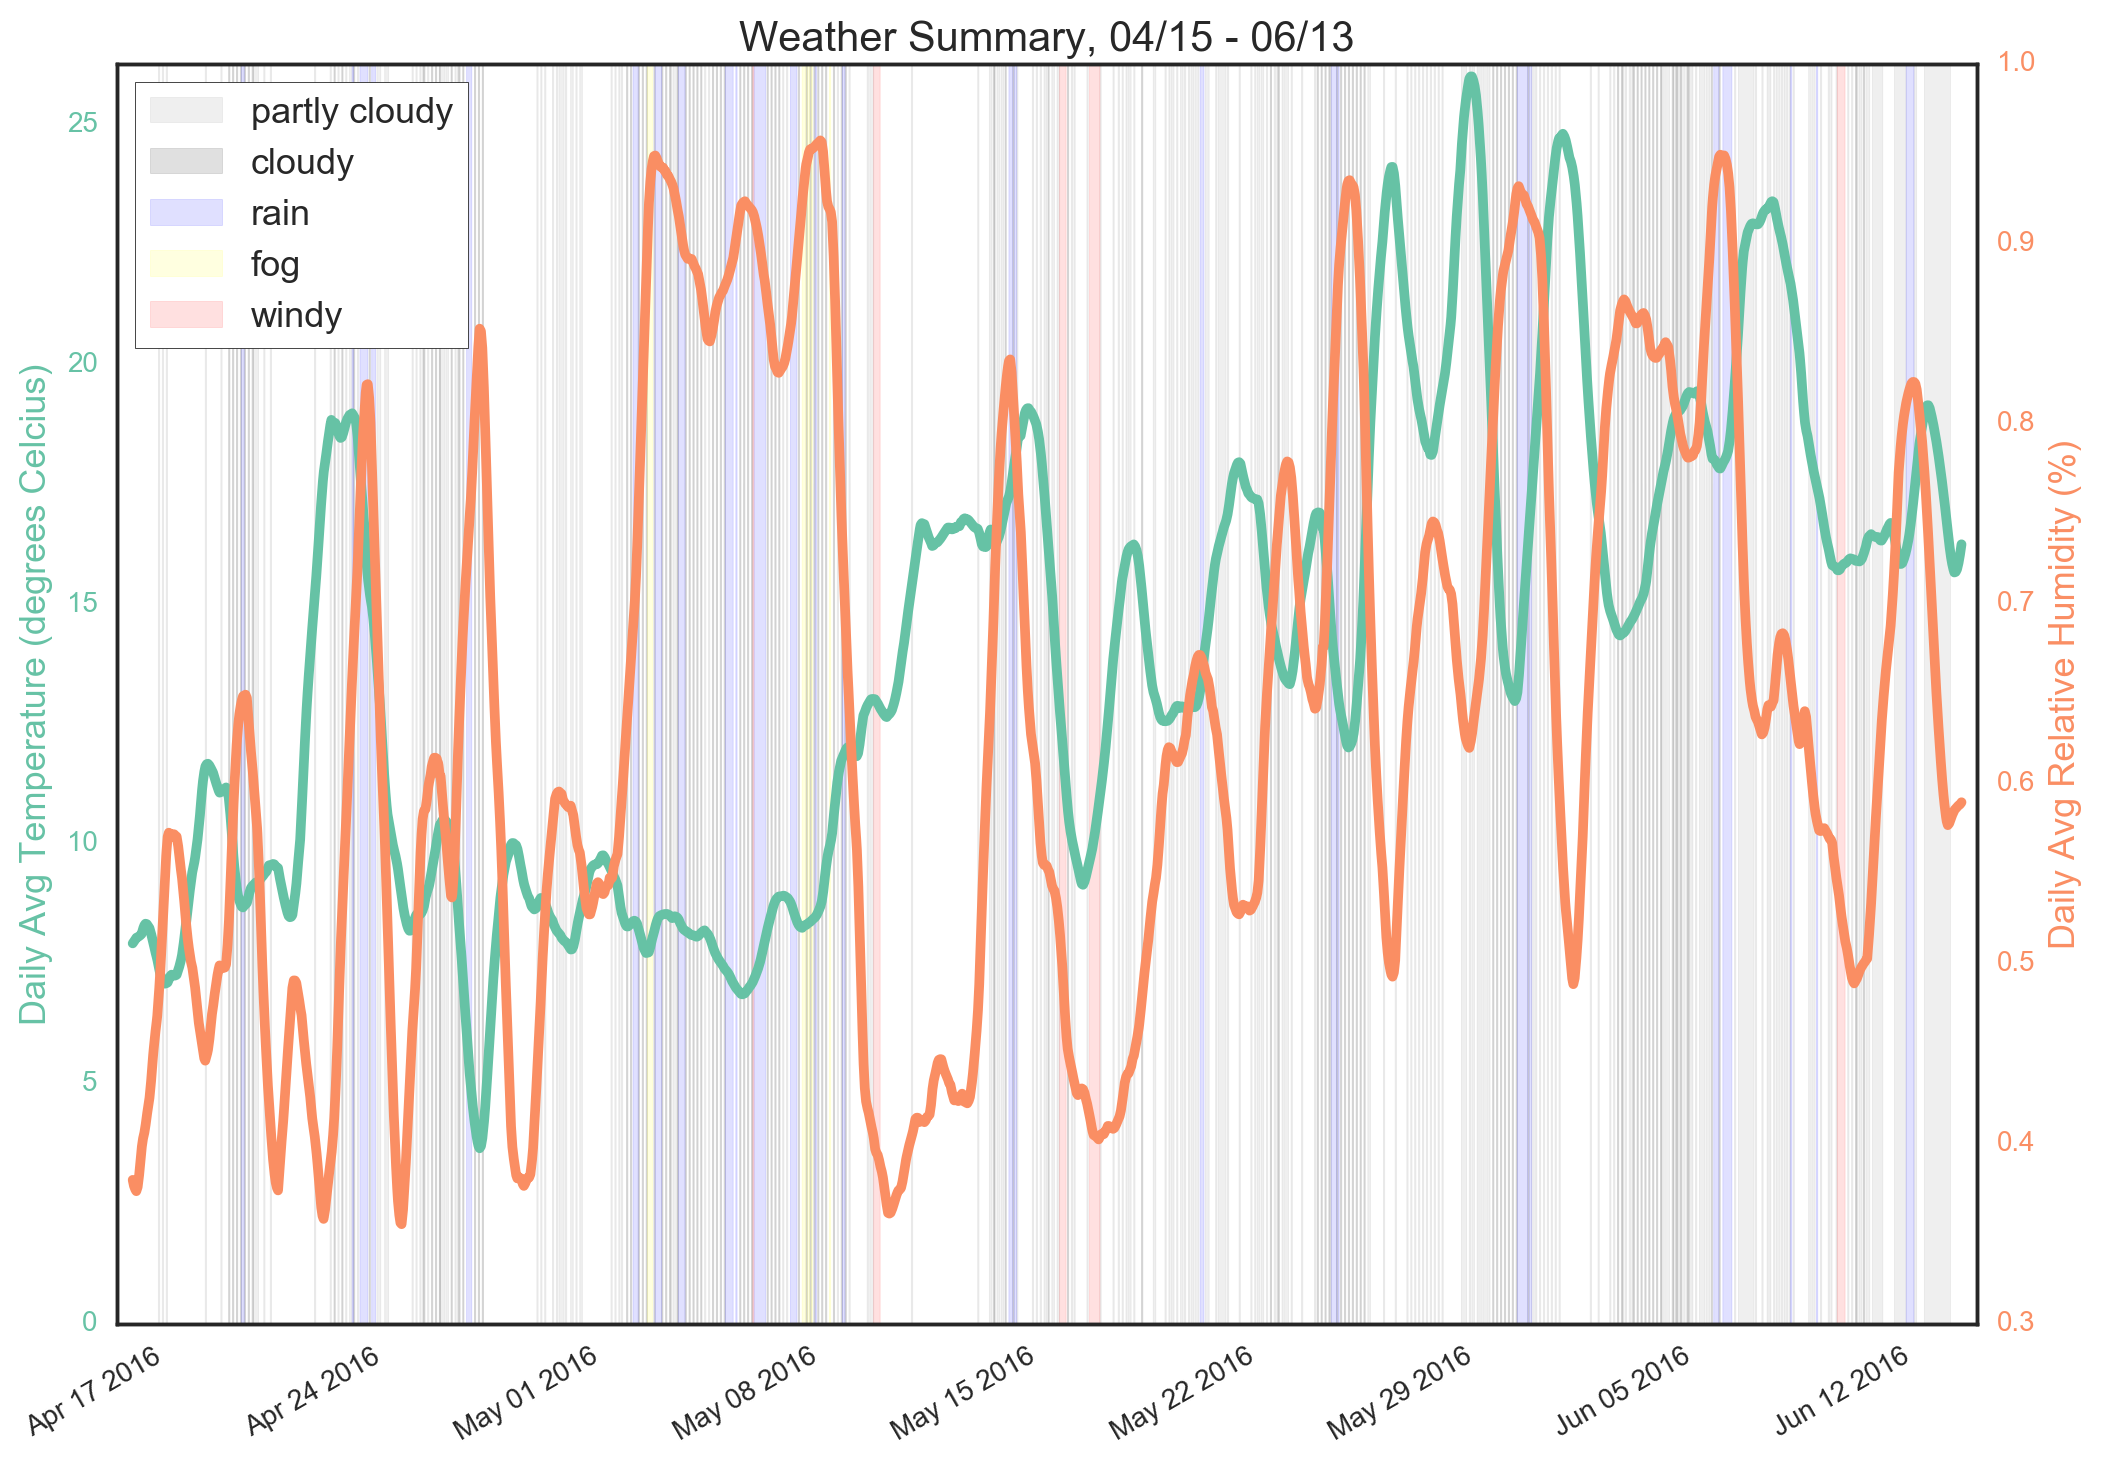
\includegraphics[width=\textwidth]{figs/weather_summary}               
 	\caption{Temperature and Humidity during Test Period.}
  	\label{fig:weather_summary}
\end{figure}
\FloatBarrier

The co-location tests started with snow on the ground and ended with summer heat.  External temperatures varied from below 5 to above 30 degrees Celcius, and the relative humidity ranged from 20-100\%.  The weather during the period was nicely varied, with a few foggy days, a few windy days, and a particularly rainy week in early May.  See Figures \ref{fig:weather} and \ref{fig:weather_summary} for details, and Appendix D for more information about trends in ambient pressure, dew, light level, precipitation amount, and cloud cover over the course of the testing period.   